%%%%%%%%%%%%%%%%%%%%%%%%%%%%%%%%%%%%%%%%%%%%%%%%%%%%%%%%%%%%%%%%%%%%%%%%%%%%%%%%
%2345678901234567890123456789012345678901234567890123456789012345678901234567890
%        1         2         3         4         5         6         7         8

\documentclass[letterpaper, 10 pt, conference]{ieeeconf}  % Comment this line out if you need a4paper

%\documentclass[a4paper, 10pt, conference]{ieeeconf}      % Use this line for a4 paper

\IEEEoverridecommandlockouts                              % This command is only needed if 
                                                          % you want to use the \thanks command

\overrideIEEEmargins                                      % Needed to meet printer requirements.

% See the \addtolength command later in the file to balance the column lengths
% on the last page of the document

% The following packages can be found on http:\\www.ctan.org
%\usepackage{graphics} % for pdf, bitmapped graphics files
%\usepackage{epsfig} % for postscript graphics files
%\usepackage{mathptmx} % assumes new font selection scheme installed
%\usepackage{times} % assumes new font selection scheme installed
%\usepackage{amsmath} % assumes amsmath package installed
%\usepackage{amssymb}  % assumes amsmath package installed

\title{\LARGE \bf
Learning Plan Refinement Graph Exploration in Combined Task and Motion Planning
}


\author{Edward Groshev$^{1}$ and Christopher Lin$^{1}$% <-this % stops a space
\thanks{$^{1}$\{\tt \small eddiegroshev, c.l\}@berkeley.edu}%
}

\input{latex_files/preamble.tex}
\input{variables.tex}

\begin{document}

\bibliographystyle{IEEEtran}

\maketitle
\thispagestyle{empty}
\pagestyle{empty}
\setlength{\textfloatsep}{8pt}% Remove \textfloatsep


%%%%%%%%%%%%%%%%%%%%%%%%%%%%%%%%%%%%%%%%%%%%%%%%%%%%%%%%%%%%%%%%%%%%%%%%%%%%%%%%
\begin{abstract}
In mobile manipulation planning, it is not uncommon for tasks to require thousands of
individual motions. Such problems require
reasoning about courses of action from the viewpoint of logical
objectives as well as the feasibility of individual movements in the
configuration space. In discrete representations, planning complexity
is exponential in the length of the plan; in mobile manipulation, the
set of parameters for an action is often continuous, so we must also
cope with an infinite branching factor. \emph{Task and motion planning} (TAMP)
methods integrate logical search with continuous geometric reasoning
to address this challenge. Our recent work in TAMP has developed a 
\emph{plan refinement graph}, a data structure which holds candidate task plans
that address different infeasibilities. The work included a preliminary technique
for learning to explore this graph. In this paper, we improve this approach,
developing techniques for using statistical machine learning and learning from demonstrations to guide the search process.
Our methods learn from human-demonstrated optimal trajectories through the space of available task plans.
Our contributions are as follows: 1) we formulate navigation through a plan
refinement graph as an MDP; 2) we present a method that trains
heuristics for intelligently searching the available space of task plans, through learning
from expert demonstrations; and 3)
we run experiments to evaluate the performance of our system. We show improvements in
performance over the systems we build on.
\end{abstract}



%%%%%%%%%%%%%%%%%%%%%%%%%%%%%%%%%%%%%%%%%%%%%%%%%%%%%%%%%%%%%%%%%%%%%%%%%%%%%%%%
\section{Introduction}
A long-term goal of robotics research is the introduction of
intelligent household robots.  To be effective, such robots will need
to perform complex tasks over long horizons (e.g., setting a dinner
table, doing laundry). Planning for these long-horizon tasks is
infeasible for state-of-the-art motion planners, making the need for a
hierarchical system of reasoning apparent.

One way to approach hierarchical planning is through combined
\emph{task and motion planning} (TAMP). In this approach, an agent is
given a symbolic, logical characterization of actions (e.g., move,
grasp, putdown), along with a geometric encoding of the
environment. TAMP systems maintain a hierarchical separation of
high-level, symbolic task planning and low-level, geometric motion
planning.  Efficient integration of these two types of reasoning is
difficult, and recent research has proposed several methods for
it~\cite{srivastava2014combined, kaelbling2011hierarchical,
  lagriffoul2014orientation, GarrettWAFR14, dornhege2012semantic}.
We adopt the principles of abstraction in the TAMP system developed by
Srivastava et al.~\cite{srivastava2014combined} (henceforth referred
to as SFRCRA-14) to factor the reasoning and search problems into
interacting logic-based and geometric components.

\begin{figure}[t]
  \centering
    \includegraphics[scale=0.17]{images/grasp_teaser_bad.png}
    \includegraphics[scale=0.17]{images/grasp_teaser_good.png}
  \caption{\small{When trying to grasp the black can, the grasping pose sampled by a robot can
significantly affect the quality of the obstructions determined. In the left image, 6 objects (shown in red) obstruct the
grasping trajectory, but in the right one, only 2 do. The new plan proposed from the right image thus only
requires moving 2 obstructions out of the way. In this work, we integrate machine learning into our task and
motion planning system using expert demonstrations, to learn an ordering on plan exploration. The system
learns to prefer simpler and more feasible plans, such as the one resulting from the scenario on the right.}}
  \label{fig:cover}
\end{figure}

Recent work~\cite{chitnis2015mlpc} that builds on SFRCRA-14 proposes
methods for jointly carrying out guided search in the space of
high-level (logic-based) plans and their low-level
\emph{refinements}, instantiations of continuous values for
symbolic references in the plan. We refer to this search for a valid low-level
refinement as \emph{plan refinement}. In this paper, we improve upon
the recent work's preliminary methods for high-level search, while retaining its methods
for learning low-level refinement distributions.

As in Chitnis et al.~\cite{chitnis2015mlpc}, we make use of unpublished work
recently submitted for review to ICRA 2016. The work develops
a \emph{plan refinement graph}, a data structure that stores a
set of qualitatively different high-level plans that could solve a task (the graph is
described in detail in Section IV-B).
During planning, we repeatedly select one such plan and either 1) try to
refine it or 2) incorporate geometric information in order to generate a new high-level
plan. This allows interleaving plan refinement with a
search over \emph{which} high-level plan to try refining, given options
that address different infeasibilities.

We present machine learning techniques used in learning from demonstrations
to train heuristic functions that guide the search process over the high level.
This amounts to learning to predict how difficult it is to refine a given plan.
Many TAMP systems rely on hand-coded heuristics to achieve this. We develop a system that uses human
demonstrations of optimal plan-space trajectories to learn intelligent navigation
of the plan refinement graph. We use 1) a max-margin formulation, which is commonly used in inverse reinforcement learning, along with Dataset Aggregation (DAgger)~\cite{ross2010dagger} and 2) a discriminative formulation using logistic regression.

The contributions of our work are as follows: 1) we formulate navigation through a plan
refinement graph as an MDP; 2) we present a method that trains
heuristics for intelligently searching the available space of task plans, through learning
from expert demonstrations; and 3)
we run experiments to evaluate the performance of our system in a
variety of simulated domains. We show improvements in performance over both SFRCRA-14
and the preliminary system developed by Chitnis et al.~\cite{chitnis2015mlpc}.

\input{related-work.tex}
\section{Background}
We provide relevant technical background and introduce notation
used throughout the paper. 

\subsection{Task and Motion Planning}

A motion planning problem is defined as a tuple $\tuple{\X, f, p_0,
  p_t}$, where $\X$ is the space of possible configurations or poses
of a robot, $f$ is a Boolean function that determines whether or not a
pose is in collision, and $p_0, p_t\in C$ are the initial and final
poses. The solution to a motion planning problem is a collision-free trajectory that
connects $p_0$ and $p_t$. To allow for object
manipulation, we let $\X$ include poses for each movable object in the
environment. 

In task and motion planning, we add more abstract concepts to this
formulation, including \emph{fluents} (logical properties that hold either
true or false and may
vary across configurations) and \emph{actions} (operations that the
agent may choose to execute, resulting in changes to the configuration
and the set of fluents that are true). Each action may require motion
planning prior to execution.  The overall problem is to plan the
sequence of actions that the agent can execute to achieve a
desired goal condition expressed in terms of fluents.

For example, we can use the action schema \emph{grasp(Object o,
  Manipulator p, GraspingPose g, Trajectory m)} to abstractly
represent grasping an object, \emph{o}.  In order to apply this action,
the agent must select values for each of these parameters (e.g.,
\emph{grasp(can$_1$, left, g$_1$, m$_1$)}). These \emph{instantiated}
actions change the value of specific fluent instantiations (also
called fluent \emph{literals}), such as \emph{in-gripper(can$_1$, gripper$_l$)}
and \emph{empty(gripper$_l$)}.

\begin{defn}
Formally, we define the task and motion planning (TAMP) problem as a tuple $\langle \Obj,
 \T, \F, \I, \G, \U \rangle$:
\begin{tightlist}
\item $\Obj$ is a set of objects denoting elements such as cans,
  trajectories, and poses. Note that $\Obj$ includes the
  configuration space of all movable objects, including the robot.
\item $\T$ is a set of object \emph{types}, such as movable objects, motion plans, poses, and locations.
\item $\F$ is a set of \emph{fluents}, which define relationships
  among objects and are Boolean functions defined over the configuration space.
\item $\I$ is the set of fluent literals that hold true in the initial state.
\item $\G$ is the set of fluent literals defining the goal condition.
\item $\U$ is a set of \emph{high-level actions} that are
  parameterized using objects and defined by \emph{preconditions}, a set
of fluent literals that must hold true in the current state to be able to perform the action;
and \emph{effects}, a set of fluent literals that hold true after the
action is performed. 
\end{tightlist}
\end{defn}

An instantiated action is said to be \emph{feasible} in a state if and only if its
preconditions hold in that state. Implicitly, the trajectories corresponding to actions
must be collision-free.

A solution to a TAMP problem is a sequence of instantiated
actions $a_{0}, a_{1}, ..., a_{n} \in \U$ such that every action is
feasible when it is applied on states successively starting with $\I$, and the
state achieved at the end of the execution sequence satisfies the
goal condition $\G$.

% As a simple example, we consider a pick domain where the robot is capable of
% performing only two actions: moving to a location and grasping an object. We can
% then specify the planning problem under our representation for the goal of holding
% a particular object $obj_{1}$ in the robot's right gripper.

% \begin{tightlist}
% \item[$\Obj$:] Objects in the environment $obj_{0}, ..., obj_{n}$, object initial poses,
% robot initial pose, and left gripper and right gripper grasping poses
% for each object. $\Obj$ is a set of symbolic references, represented at the high
% level only as strings with no geometric interpretation.

% \item[$\F$:] \emph{Obstructs}$(traj, obj_{0}, obj_{1})$, \emph{InGripper}$(obj, gripper)$,\\\emph{Empty}$(gripper)$,
% \emph{IsGraspPose}$(pose, obj, gripper)$,\\\emph{At}$(obj, pose)$, \emph{RobotAt}$(pose)$,\\
% \emph{IsValidTraj}$(traj, pose_{0}, pose_{1})$. Here, the \emph{IsValidTraj} predicate checks that $traj$
% joins $pose_{0}$ with $pose_{1}$, and that it is feasible to execute and
% collision-free.

% \item[$\I$:] \emph{IsGraspPose} between all grasping poses and their corresponding object,
% \emph{RobotAt} the robot's initial pose, \emph{At} for all object initial poses, and
% \emph{Empty} for both grippers.

% \item[$\G$:] \emph{InGripper}$(obj_{1}, right\_gripper)$.

% \item[$\U$:]
% \begin{tightlist}
% \item[1)] \emph{MoveTo}
%   \begin{tightlist}
%   \item[params:]$pose_{0}, pose_{1}, traj$
%   \item[preconds:]\emph{RobotAt}$(pose_{0}) \wedge$\\ \emph{IsValidTraj}$(traj, pose_{0}, pose_{1})$
%   \item[effects:]\emph{RobotAt}$(pose_{1}) \wedge \lnot$\emph{RobotAt}$(pose_{0})$
%   \end{tightlist}
% \item[2)] \emph{Grasp}
%   \begin{tightlist}
%   \item[params:]$obj, obj\_pose, robot\_pose,\\grasp\_pose, gripper, traj$
%   \item[preconds:]\emph{RobotAt}$(robot\_pose) \wedge$\\ \emph{Empty}$(gripper) \wedge$
% \emph{At}$(obj, obj\_pose) \wedge$\\ \emph{IsGraspPose}$(grasp\_pose, obj, gripper) \wedge$\\ \emph{IsValidTraj}$(traj, robot\_pose, grasp\_pose)$
%   \item[effects:]\emph{RobotAt}$(grasp\_pose) \wedge$ $\lnot$\emph{RobotAt}$(robot\_pose) \wedge \lnot$\emph{Empty}$(gripper) \wedge\\
% \lnot$\emph{At}$(obj, obj\_pose) \wedge$ \emph{InGripper}$(obj, gripper) \wedge \forall\ traj', o: \lnot$\emph{Obstructs}$(traj', obj, o)$
%   \end{tightlist}
% \end{tightlist}
% \end{tightlist}

% For the \emph{Grasp} action, the fact that the path to $obj$ must be collision-free is
% implicitly checked within the \emph{IsValidTraj} precondition. An important aspect of
% this formulation is the assumption that grasping an object causes it to no longer
% obstruct any other object in the environment. If no other object obstructs $obj_{1}$,
% a possible high-level plan with a feasible refinement for achieving $\G$ is
% \begin{tightlist}
% \item[1.] \emph{MoveTo}$(robot\_init\_pose, rgripper\_bp\_obj_{1})$
% \item[2.] \emph{Grasp}$(obj_{1}, obj_{1}\_init\_pose, rgripper\_bp\_obj_{1},\\rgripper\_gp\_obj_{1}, rgripper)$
% \end{tightlist}

% The $bp$ parameters refer to robot base poses in preparation for grasping an object.
% The trajectory parameters are not included here because they are based on the interface layer's
% sampling of the base pose and grasping pose. If $obj_{1}$ is
% obstructed by, say, $obj_{3}$ in the environment, a possible high-level plan would involve
% grasping first $obj_{3}$ then $obj_{1}$.




% For example, consider the previous pick domain specification where $obj_{3}$ does obstruct $obj_{1}$.
% Initially, the task planner returns a high-level plan to immediately grasp $obj_{1}$, because
% it is not yet aware of the obstruction. The interface layer then samples grasp poses
% for $obj_{1}$, but motion planning for each sample fails due to the obstruction. Eventually,
% this error is propagated back to the task planner. The new high-level plan correctly
% grasps $obj_{3}$ before $obj_{1}$, and refining this plan succeeds.

% For example, consider a pick domain with two objects: a target $o_{t}$ to be grasped and an obstruction.
% Initially, the task planner returns a high-level plan to immediately grasp $o_{t}$, because
% it is not yet aware of the obstruction. The interface layer then samples grasp poses
% for $o_{t}$, but motion planning for each sample fails due to the obstruction. Eventually,
% this error information about the obstruction is converted into a symbolic representation
% and propagated back to the task planner. The new high-level plan correctly grasps the obstruction
% before grasping $o_{t}$, and refining this plan succeeds.

\subsection{Markov Decision Processes}
Markov decision processes (MDPs) provide a way to formalize
interactions between agents and environments. At each step of an MDP,
the agent knows its current state and selects an action. This causes the
state to change according to a known transition distribution.
\begin{defn}
Formally, we define an MDP as a tuple $\langle \St, \A, T, R, \gamma, \Prob \rangle$, where
\begin{tightlist}
\item $\St$ is the state space.
\item $\A$ is the action space.
\item $T(s, a, s') = Pr(s' | s, a)$ for $s, s' \in \St, a \in \A$ is the transition distribution.
\item $R(s, a, s')$ for $s, s' \in \St, a \in \A$ is the reward function.
\item $\gamma \in [0, 1]$ is the discount factor.
\item $\Prob$ is the initial state distribution.
\end{tightlist}
\end{defn}
A solution to an MDP is a policy, $\pi: \St \rightarrow \A$, that maps states to
actions. The value, $V_{\pi}(s)$, of a state under $\pi$ is the sum of expected
discounted future rewards generated from starting in state $s$ and selecting actions according
to $\pi$:
$$V_{\pi}(s) = \mathbb{E}[\sum_{t=0}^{\infty}\gamma^{t}R(s_{t}) | \pi, s_{0} = s].$$
The optimal policy, $\pi^{*}$, maximizes this value for all states.

\section{Solving Task and Motion Planning Problems}
\begin{figure}[t]
  \centering
    \includegraphics[scale=0.3]{images/ex_prg.png}
  \caption{\small{A simple plan refinement graph for an environment with 3 objects: A,
B, and C. The goal is to grasp object A. Each node maintains a high-level
plan and a set of instantiated continuous values for its symbolic references.
The edges are labeled with errors discovered by the low-level motion planner and
propagated back up to the task planner for replanning.}}
  \label{fig:prg}
\end{figure}

\subsection{SFRCRA-14}
Solving TAMP problems requires evaluation of
possible courses of action comprised of different combinations of
instantiated action operators. This is particularly challenging
because the set of possible action instantiations (and thus the
branching factor of the underlying search problem) is infinite.
We give a brief overview of SFRCRA-14, a recent approach to TAMP, and
refer the interested reader to the cited paper for further details.

SFRCRA-14 solves TAMP problems by: incrementally
searching for a high-level plan that solves the logical abstraction
of the given TAMP problem; determining a prefix of the plan that has a
motion planning feasible refinement; updating the high-level
abstraction to reflect the reason for infeasibility; and searching for
a new plan suffix from the failure step onwards. This search process
addresses the fundamental TAMP problem: high-level
logical descriptions are lossy abstractions of the true environment
dynamics and thus may not include sufficient information to
determine the true applicability of a sequence of actions.

In general, including geometric properties in the logic-based formulation leads to an
increase in the number of objects representing distinct poses and/or trajectories. For
instance, expressing the fact that a trajectory for grasping \emph{can$_1$} is obstructed by
\emph{can$_3$} from the current pose of the robot would require setting a fluent of the
form \emph{obstructs(can$_3$, pose$_{17877}$, trajectory$_{3219}$, can$_1$)} to true in
the description of the high-level state. In turn, this would require adding
\emph{pose$_{17877}$} and \emph{trajectory$_{3219}$} into the set of objects if they were
not already included. Unfortunately, the size of the abstracted, logic-based state space
grows exponentially with the number of objects, and such an approach quickly leads to
unsolvable task planning problems.

SFRCRA-14 addresses this challenge by abstracting the continuous
action arguments, such as robot grasping poses and trajectories, into
a \emph{bounded} set of symbolic references to potential values. A
\emph{high-level}, or \emph{symbolic}, plan refers to the fixed task
sequence returned by a task planner and comprised of these symbolic
references. An \emph{interface layer} conducts plan refinement,
searching for instantiations of continuous values for symbolic
references while ensuring action feasibility.  The resulting process
is able to utilize off-the-shelf task and motion planners while
carrying out the necessary exchange of information in a scalable
manner.

\subsection{Plan Refinement Graph}
Unpublished work recently submitted for review to ICRA 2016 builds on SFRCRA-14 and develops a complete algorithm
that maintains a \emph{plan refinement graph} (PRGraph). Every node $u$ in the PRGraph
represents a high-level plan $\pi_u$ and the current state of the search
for a refinement. An edge $(u,v)$ in the PRGraph
represents a ``correction'' of $\pi_u$ for a specific instantiation of
the symbolic references in $\pi_u$. Let $\pi_{u,k}$ be the plan prefix of
$\pi_u$ consisting of the first $k$ actions. Formally, each edge
$e=(u,v)$ is labeled with a tuple $\langle \sigma, k, \varphi \rangle$.
$\sigma$ denotes an instantiation of references for a prefix $\pi_{u,k}$ of
$\pi_u$ such that feasible motion plans have been found for all
previous actions $\pi_{u,k-1}$. $\varphi$ denotes a conjunctive formula
consisting of fluent literals
that were required in the preconditions of the $k^{th}$ action in
$\pi_u$ but were not true in the state obtained upon
application of $\pi_{u,k-1}$ with the instantiation $\sigma_k$.  The
plan in node $v$ (if any) retains the prefix $\pi_{u,k-1}$ and solves
the new high-level problem which incorporates the discovered facts $\varphi_{u,v}$
in the $k^{th}$ state.

The overall search algorithm then interleaves the search for feasible
refinements of each high-level plan with the addition into the
PRGraph of new edges and plan nodes using the semantics described above.

\figref{fig:prg} illustrates a simple example of a PRGraph.

\subsection{Previous Approach for Learning to Search the PRGraph}
Chitnis et al.~\cite{chitnis2015mlpc} explain that the high level has a two-tiered
decision to make: which node in the PRGraph to
visit next, and whether to 1) attempt to refine this node or 2) quickly generate failure information
from it, thus spawning a child node. They develop heuristics that are trained to estimate
the difficulty associated with refining a plan, in order to make this decision intelligently.

To select among the potential refinement options, the authors train two decision tree regressors
that determine how many iterations would be needed to achieve a valid refinement for a node, or for a child
of that node which incorporates a single additional geometric fact about the environment.
To obtain an estimate for a full plan, they sum this number across all of the plan's actions.
The implicit assumption being made here is that dependencies in plans are, in some way, local:
the plan must be factorizable into subportions with independent refinements.

At test time, they use the regressors to find the best two-tiered action to take at each step.
For example, if refining a child node would reduce the number of steps to a valid refinement,
they bias toward generating a child node.
\section{Learning to Search the PRGraph}
\subsection{Formulation as MDP}
We adopt the same two-tiered decision strategy described in Section IV-C.
We formulate PRGraph search as an MDP as follows:
\begin{tightlist}
\item A state $s \in \St$ is a tuple $(PRG, r_{cur}, E)$, consisting of the
PRGraph with all its high-level plans, the current setting of
values for symbolic references for all high-level plans, and
an encoding of the geometric environment.
\item An action $a \in \A$ is a pair $(n, m)$, where $n$ is the selected node and $m$ is
the mode to apply (either trying to refine the node or quickly generating failure information).
\item If we select a node $n$ to try to refine, the transition function $T(s, a, s')$ is the same
as that in the plan refinement MDP presented in Chitnis et al.~\cite{chitnis2015mlpc} Briefly,
it describes how continuous values for symbolic references in node $n$'s plan are resampled, altering $r_{cur}$. If we instead
try to quickly generate failure information for $n$, then $T$ is defined by how we determine a geometric
fact to replan with at the task planner level. In our system, we sample a trajectory (which may have
collisions) for achieving each step in the plan, then roll out that trajectory in simulation and propagate
back to the task planner the first error we encounter (obstructing object, unreachable object, etc.).
\item The reward function $R(s, a, s')$ is 1 if $r_{cur}$ for any high-level plan in the PRGraph
has collision-free linking trajectories, and 0 otherwise.
\end{tightlist}

\subsection{Max-Margin Approach}
We exploit properties of the environment to hand-design a feature vector $f(n)$ that geometrically
describes aspects of a single high-level plan, thus encoding its refinability. Because the mode $m$ is binary,
we construct $$f((n, m)) = \begin{bmatrix} f(n) \\ f(n) \end{bmatrix}^\top \begin{bmatrix} 1 - m \\ m \end{bmatrix},$$
which stacks the feature vector for $n$ on itself, then turns off the bottom half when $m = 0$ and the
top half when $m = 1$. Now that we have defined a feature vector associated with each action that can be taken
from a state, we can obtain human-demonstrated trajectories (sequences of actions $(n, m)^{*}$) that intelligently
navigate the PRGraph. We then solve the following max-margin optimization problem with a structured margin and slack variables:
$$\min ||w||^{2} + C\sum_{i} \xi_{i}$$
$$\text{s.t.}\ w^{\top}f((n, m)_{i}^{*}) \geq w^{\top}f((n, m)_{ij}) + $$
$$d(f((n, m)_{i}^{*}), f((n, m)_{ij})) - \xi_{i}\ \forall i, j,\ \xi_{i} \geq 0\ \forall i$$
where the $i$ iterate over the demonstrated trajectories and the $j$ iterate over possible actions. Each
demonstrated trajectory has an associated slack variable in this formulation.
We note that the weight vector $w$ encodes a score function on the different actions, which produces
an ordering that matches the Q-function in the described MDP. Of course, the score function is not identical
to the Q-function, because we are not incorporating $R(s, a, s')$ in our formulation for $w$.

We use DAgger to augment our training data. In the first iteration, we navigate the PRGraph following
the expert actions and store these actions in a dataset. After some iterations, we use the dataset to solve for an
initial weight vector $w$. On subsequent iterations, we navigate the PRGraph by rolling out the policy
encoded by $w$ (pick the action with the highest score $w^{\top}f((n, m))$) while asking the expert what
the optimal action would be at each step, appending these into the dataset. After some iterations, we use the
aggregated dataset to solve for a new $w$, and repeat.

At test time, we follow the policy encoded by $w$ straightforwardly, picking the highest-scoring action
at each step.

\subsection{Logistic Regression Approach}
Within the framework of classification, a policy can be viewed as a classifier that discriminates between ``good'' and ``bad'' actions. While it is natural to model the quantity $p(action|state)$, which can be viewed as a multi-class classification problem, the action space support varies with the number of nodes added to the PRGraph. Instead, we relax the problem and model the quantity $p(optimal|action,state)$. This is simply a binary classification problem where the label takes on two possible values: ``optimal'' and ``not optimal''. Using a logistic regression model we express the conditional probability as $$p(optimal=true|action,state;w) = \frac{1}{1+e^{-w^\top x}}$$ where $x = f((n,m))$ is the feature vector associated with the current action. To estimate the parameter vector $w$ we minimize the following cost function: $$\ell(w|D)=\lambda||w||^2_2-\sum_{ij} y_{ij}\log\mu_{ij}+(1-y_{ij})\log(1-\mu_{ij})$$ where $\mu_{ij}=1/(1+e^{-w^\top f((n,m)_{ij})})$ and $y_{ij}=1$ if the human took action $j$ in the $i$'th demonstration and $0$ otherwise. We make the assumption that humans performs optimally.

For this approach we do not explicitly use DAgger to augment the training data, instead we train on the largest data set that was collected. At test time, we evaluate a stochastic policy and a deterministic policy. The deterministic policy takes the action with the highest probability of being optimal. For the stochastic policy we normalize the probability of being optimal across all possible actions and randomly select an action from the resulting distribution.
\section{Experiments}
\begin{figure}[t]
  \centering
    \includegraphics[scale=0.3,angle=90]{images/feature_cone.png}
  \caption{\small{If the target object to be grasped is the black can, we consider the objects
whose centers lie in a cone from angles $-\frac{\pi}{3}$ to $\frac{\pi}{3}$ toward the closest table edge in
our feature computations. These objects are shown here in red.}}
  \label{fig:cone}
\end{figure}

\begin{table}[h!]
  \centering
  \vspace{8pt}
  \tabcolsep=0.11cm{
  \begin{tabular}{ccccc}
    \toprule[1.5pt]
      \textbf{\# Cans} & \textbf{System} & \textbf{\% Solved} & \textbf{Avg Time (s)} & \textbf{Avg \# MP Calls}\\
    \midrule[2pt]
      25 & B1 & 96 & 28.7 & 22\\
    \midrule
      25 & B2 & 98 & 30.0 & 21\\
    \midrule
      25 & I0 & 94 & 24.8 & 21\\
    \midrule
      25 & I1 & 94 & 28.5 & 19\\
    \midrule
      25 & I2 & 100 & 21.0 & 18\\
    \midrule
      25 & LS & 96 & 29.1 & 23\\
    \midrule
      25 & LD & 98 & 19.8 & 18\\
    \midrule[1.5pt]
      30 & B1 & 74 & 48.9 & 29\\
    \midrule
      30 & B2 & 80 & 48.0 & 29\\
    \midrule
      30 & I0 & 72 & 40.0 & 29\\
    \midrule
      30 & I1 & 76 & 44.2 & 28\\
    \midrule
      30 & I2 & 80 & 42.7 & 30\\
    \midrule
      30 & LS & 78 & 45.7 & 35\\
    \midrule
      30 & LD & 78 & 37.8 & 29\\
    \midrule[1.5pt]
      35 & B1 & 68 & 24.5 & 15\\
    \midrule
      35 & B2 & 72 & 29.7 & 15\\
    \midrule
      35 & I0 & 74 & 31.1 & 15\\
    \midrule
      35 & I1 & 76 & 22.4 & 14\\
    \midrule
      35 & I2 & 80 & 22.7 & 14\\
    \midrule
      35 & LS & 76 & 23.5 & 15\\
    \midrule
      35 & LD & 82 & 25.5 & 15\\
    \midrule[1.5pt]
      40 & B1 & 58 & 35.9 & 15\\
    \midrule
      40 & B2 & 64 & 48.0 & 19\\
    \midrule
      40 & I0 & 58 & 54.5 & 22\\
    \midrule
      40 & I1 & 64 & 36.6 & 14\\
    \midrule
      40 & I2 & 76 & 36.9 & 16\\
    \midrule
      40 & LS & 64 & 51 & 22\\
    \midrule
      40 & LD & 70 & 49.1 & 18\\
    \bottomrule[1.5pt]
  \end{tabular}}
  \caption{\small{Percent solved, average overall time, and average number of calls to the motion
planner for baseline 1 (B1), baseline 2 (B2), logistic regression with stochastic policy (LS), logistic regression with deterministic policy (LD), and max-margin with DAgger after iteration 0 (I0), 1 (I1), and 2 (I2).
Iteration 0 evaluates performance before DAgger was run (so just the initial set of 100 demonstrations),
and iterations 1 and 2 are after one and two rounds of DAgger, respectively. Average time and number of
motion planner calls were computed across the subset of environments for which all systems succeeded, which
explains why they do not scale with the number of cans. Time limit: 300s.}}
  \label{table:results}
  % \vspace{-1em}
\end{table}

We evaluate our approach in the can domain, which has cans uniformly distributed on a table. We
compare performance with two baselines. Baseline 1 is SFRCRA-14, which uses the
following fixed graph search policy: try 3 times to refine the deepest
node in the PRGraph; if unsuccessful, generate a geometric fact from it, replan (which
creates a child node), and repeat. The number 3 was chosen to trade off between providing
each node a fair opportunity to be refined (which could fail a couple of times if sampling produces
undesirable values), and not spending too much time before giving up and generating a child node to try next.
Baseline 2 is the prior work by Chitnis et al.~\cite{chitnis2015mlpc}, described in Section IV-C.

\begin{figure}[h]
  \centering
    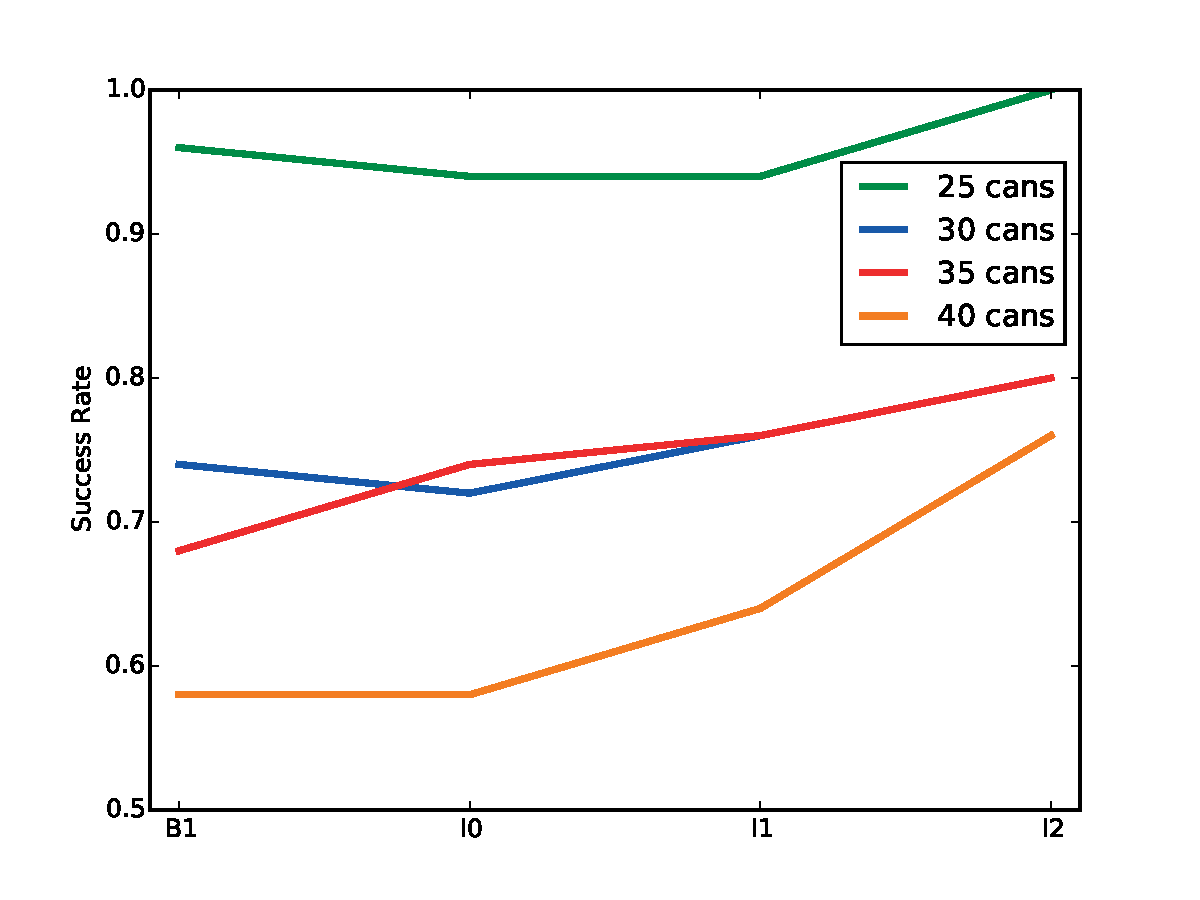
\includegraphics[scale=0.43]{images/results_line}
  \caption{\small{Line graph illustrating success rates on the test set for baseline 1
and our system after each round of DAgger, using the abbreviations described in the
table caption. Our method performs much better than the baseline after 2 iterations of DAgger.
We also note the upward trend in success rate across the iterations.}}
  \label{fig:results_line}
\end{figure}

\begin{figure}[h]
  \centering
    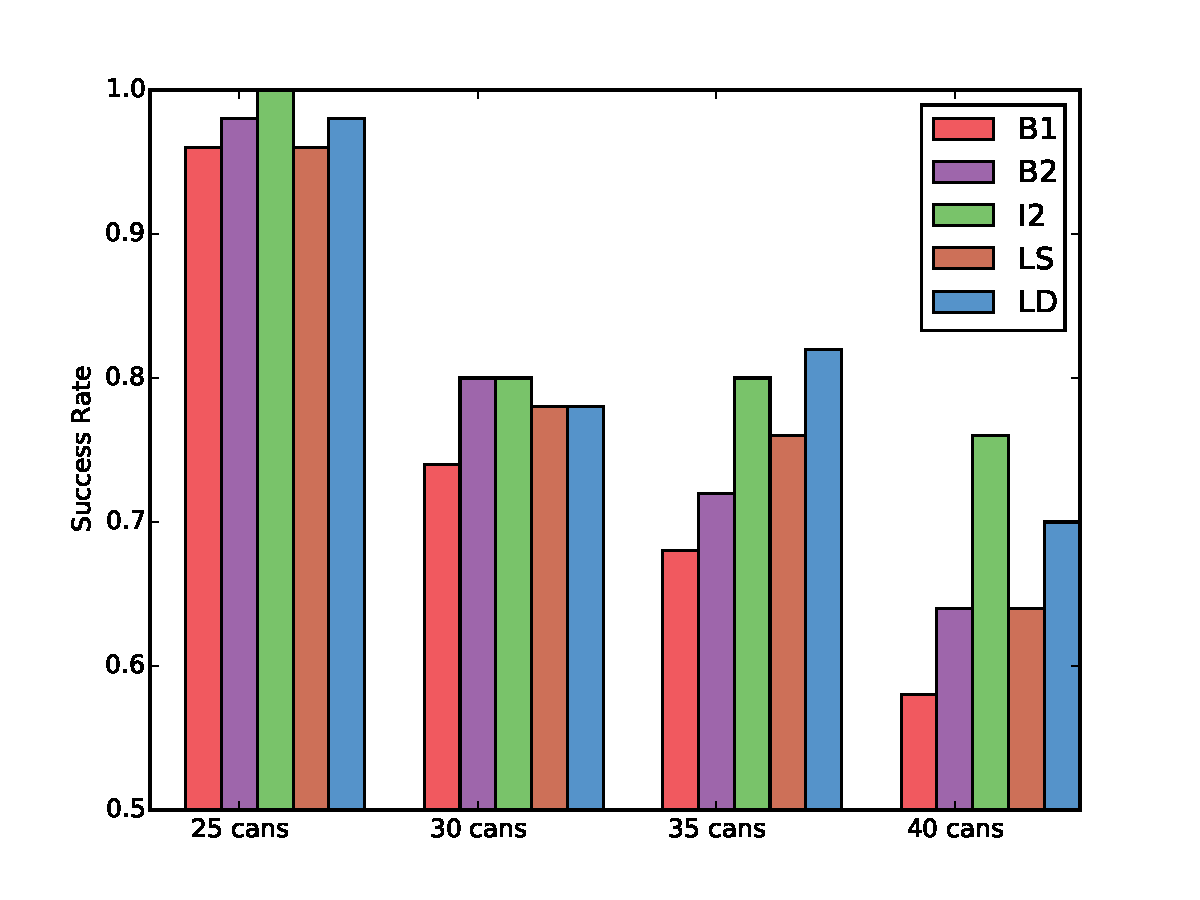
\includegraphics[scale=0.43]{images/results_bar_succ}
  \caption{\small{Bar graph illustrating success rates on the test set for the
two baselines, the two logistic regression policies, and our max-margin formulation after 2 iterations of DAgger. The abbreviations are described in the caption of Table I. The max-margin approach achieved much higher
success rates than both baselines, in general. The deterministic policy trained with logistic regression had comparable results.}}
  \label{fig:results_bar_succ}
\end{figure}

\begin{figure}[h]
  \centering
    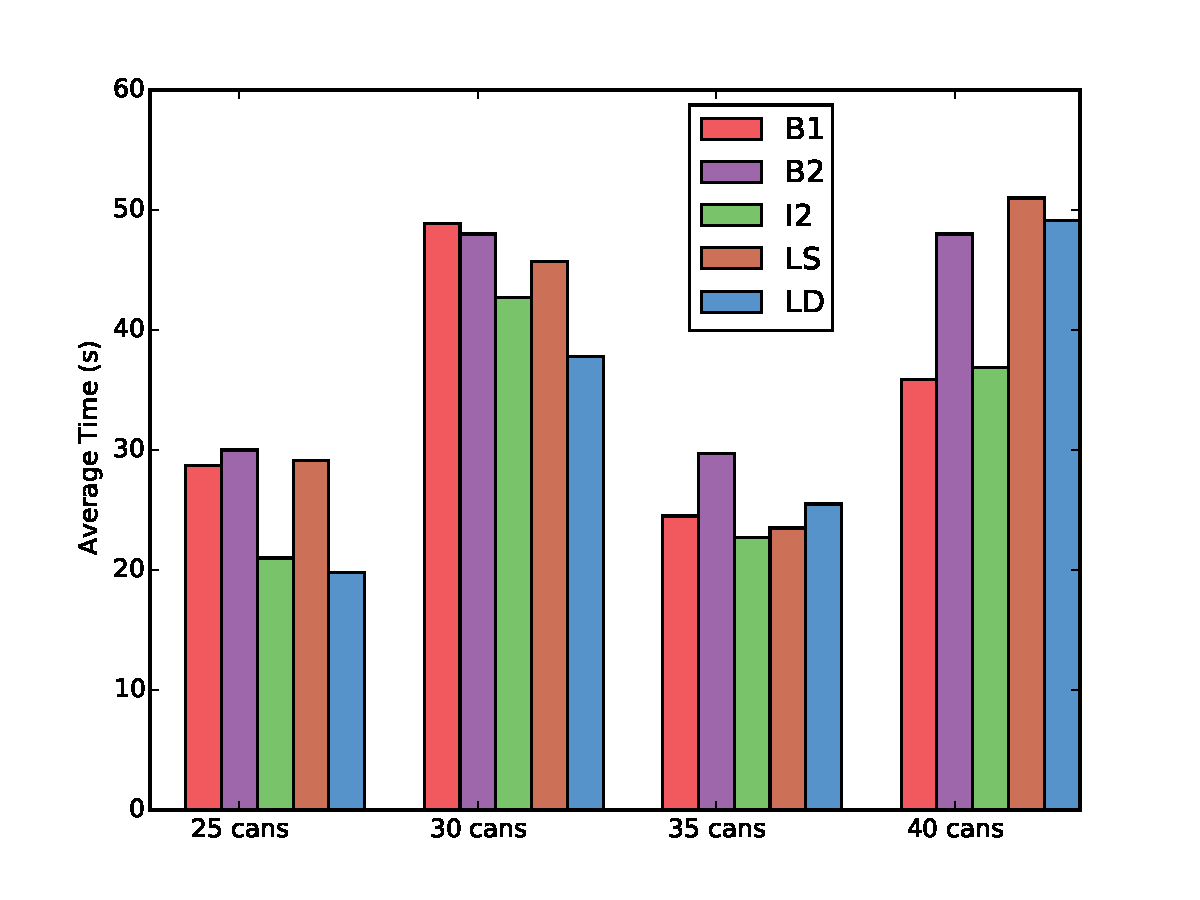
\includegraphics[scale=0.43]{images/results_bar_time}
  \caption{\small{Bar graph illustrating average total times on the test set for the
two baselines, the two logistic regression policies, and our max-margin formulation after 2 iterations of DAgger. The abbreviations are described in the caption of Table I. The max-margin approach produced noticeably faster
performance than both baselines, in general. The deterministic policy trained with logistic regression had comparable results. In the 40 can environment it had an increased planning time compared to the baseline, but this is OK because in more challenging environments the baseline can only solve simple instantiations which naturally have a lower planning time.}}
  \label{fig:results_bar_time}
\end{figure}

We run four sets of experiments, using 25, 30, 35, and 40 cans on the table.
The goal across all experiments is for the robot to pick up a particular object with its
left gripper. We disabled the right gripper, so any obstructions to the target object must be picked up and
placed elsewhere on the table. This domain has 4 types of continuous references: base poses, object grasp
poses, object putdown poses, and object putdown locations onto the table.

We now describe the feature vector $f(n)$ associated with a high-level plan. Because the plan is composed
of a sequence of object grasp and putdown actions, we first consider features of a single grasp action, targeted
at an object $o$ in the environment. Consider a cone ranging from angles $-\frac{\pi}{3}$ to $\frac{\pi}{3}$
toward the closest table edge from $o$, as shown in \figref{fig:cone}. The first feature, exists\_obstr, is a binary variable indicating
whether any other objects lie in this cone. The second, exists\_path, is a binary variable indicating whether there is a linear
grasp path wide enough for the robot's gripper to fit through within the cone. For the third feature, we approximate the robot's arm and gripper with a cylinder $c$ and sweep it across 10 discretized angles from $-\frac{\pi}{3}$ to
$\frac{\pi}{3}$. We then store the minimum number of collisions with $c$ as the feature, sweep\_count. This gives us a coarse approximation for the minimum number of object that should be moved before the target object is accessible via a linear path.
% We store this value as the third feature, sweep\_count. The third, sweep\_count, sweeps
% a cylinder $c$ approximating the robot's gripper across 10 discretized angles from $-\frac{\pi}{3}$ to
% $\frac{\pi}{3}$ and is the minimum number of objects in collision with $c$ across these angles.
We construct these features for the first five grasp actions in the plan (padding with -1 if there are not enough).
We then add on the following aggregate features associated with the entire plan: 1) the minimum exists\_obstr across all grasp actions,
2) the sum of sweep\_count across all grasp actions, 3) a counter for how many times $n$ was picked for refinement,
4) a counter for how many times $n$ was picked for generating an error,
5) the max of 0 and the difference between expected plan length and the current plan length, this indicates how much shorter the current plan is, and 6) the analog of the previous feature to indicate how much longer than expected the current plan is. The expected plan length is approximated as a linear function of sweep\_count. For the logistic regression approach we added a bias term to the feature vector.

We report results on fixed test sets of 50 randomly generated environments per number of objects. At each
iteration of training, we collect approximately 100 optimal actions from the human demonstrator (using
DAgger, this means collect 100 demonstrations, construct $w$, collect 100 more while rolling out $w$, construct new $w$, repeat).
We found that after 2 rounds of DAgger, performance plateaued, so we stopped there.

Our experiments are conducted in Python 2.7 using the OpenRave simulator~\cite{Diankov_2008_6117} with a PR2 robot.
The motion planner we use is trajopt~\cite{schulman2013finding}, and the task planner is Fast-Forward~\cite{FF}.
The experiments were carried out in series on an Intel Core i7-4770K machine with 16GB RAM. For the max-margin optimization,
we used a constant margin of $d = 1$, and we set $C = 10^{9}$, indicating that we want to penalize violating
constraints significantly and are willing to have $||w||$ grow. In our experiments, though, $||w||$ did not actually become
so large that overfitting was an issue. We used Gurobi for solving the quadratic program.

Table \ref{table:results} summarizes our quantitative results. \figref{fig:cover} illustrates a scenario where
our learning methods prove important. \figref{fig:results_line}, \figref{fig:results_bar_succ}, and \figref{fig:results_bar_time} show our quantitative
results in graphs. The results demonstrate significant improvements in performance to the baseline systems for success rate and
average overall time. The number of calls to the motion planner remained roughly the same,
suggesting that the performance benefits instead derive from less time wasted on inverse kinematics checks when
attempting to refine plans with no valid refinement.

\input{conclusion.tex}
\section{Acknowledgements}
We thank Eddie Groshev and Dylan Hadfield-Menell for their collaboration, advice, and feedback
throughout this project.

%\addtolength{\textheight}{-12cm}   % This command serves to balance the column lengths
                                  % on the last page of the document manually. It shortens
                                  % the textheight of the last page by a suitable amount.
                                  % This command does not take effect until the next page
                                  % so it should come on the page before the last. Make
                                  % sure that you do not shorten the textheight too much.

%%%%%%%%%%%%%%%%%%%%%%%%%%%%%%%%%%%%%%%%%%%%%%%%%%%%%%%%%%%%%%%%%%%%%%%%%%%%%%%%



%%%%%%%%%%%%%%%%%%%%%%%%%%%%%%%%%%%%%%%%%%%%%%%%%%%%%%%%%%%%%%%%%%%%%%%%%%%%%%%%



%%%%%%%%%%%%%%%%%%%%%%%%%%%%%%%%%%%%%%%%%%%%%%%%%%%%%%%%%%%%%%%%%%%%%%%%%%%%%%%%
\bibliography{latex_files/references}

\end{document}
